\documentclass[conference]{IEEEtran}
\IEEEoverridecommandlockouts
% The preceding line is only needed to identify funding in the first footnote. If that is unneeded, please comment it out.
%Template version as of 6/27/2024

\usepackage{cite}
\usepackage{amsmath,amssymb,amsfonts}
\usepackage{algorithmic}
\usepackage{graphicx}
\usepackage{textcomp}
\usepackage{xcolor}
\def\BibTeX{{\rm B\kern-.05em{\sc i\kern-.025em b}\kern-.08em
    T\kern-.1667em\lower.7ex\hbox{E}\kern-.125emX}}
\begin{document}

\title{A Comparative Analysis of ResNet and EfficientNet Architectures for Fine-Grained Vehicle Classification}

\author{\IEEEauthorblockN{1\textsuperscript{st} Gabriel Pires e Peixotto}
\IEEEauthorblockA{\textit{INF} \\
\textit{UFRGS}\\
Porto Alegre, Brazil \\
gpp.gabrielpires@gmail.com}}

\maketitle

\begin{abstract}
Fine-grained image classification is a challenging task because inter-class differences are often minimal, while intra-class variance can be high due to angles and lighting. This paper presents a comparative analysis of two popular Convolutional Neural Networks, ResNet50 and EfficientNet-B4, on the Stanford Cars dataset (196 classes). A custom pre-processing technique called letterboxing is detailed to preserve the aspect ratio of vehicles, and a two-phase transfer learning approach is employed to prevent overfitting. Under a strict 40-epoch training limit, results show that EfficientNet-B4 outperforms ResNet50, achieving an accuracy of 82.39\% compared to 80.59\%. Additionally, through Grad-CAM interpretability analysis, an unexpected ``padding artifact'' phenomenon is revealed, demonstrating that the models exploit the artificial black borders as a geometric shortcut to infer the original aspect ratio of the vehicles.
\end{abstract}

\begin{IEEEkeywords}
Fine-Grained Visual Categorization, Deep Learning, ResNet, EfficientNet, Grad-CAM, Transfer Learning
\end{IEEEkeywords}

\section{Introduction}
Image classification usually involves telling apart very different objects, like cats and airplanes. However, Fine-Grained Visual Categorization (FGVC) is a harder task. It tries to distinguish between very similar sub-categories within the same group. A classic example is the Stanford Cars dataset, which has 196 specific vehicle classes. Here, a model must learn to tell the difference between cars of the same brand and model but from different years, like a 2007 Bentley versus a 2012 Bentley.

This task is hard because cars from different classes often look very similar (low inter-class variance), while cars from the exact same class can look different depending on the camera angle, lighting, or background (high intra-class variance). To work well, the models cannot just look at the general shape of a car. They need to find small, specific details, such as the shape of a headlight or the style of a front grille.

This project compares two popular Convolutional Neural Network (CNN) architectures on the Stanford Cars dataset: ResNet50 and EfficientNet-B4. ResNet50 is a common baseline model, while EfficientNet-B4 is a more modern approach that balances depth, width, and image resolution for better performance. The objective is to see how well each model learns these small details when trained on a consumer GPU. A tool called Grad-CAM is also used to see exactly where the models are looking. This helps in understanding how image cropping and padding steps affect what the models learn.


\section{Related Work and State of the Art}
The Stanford Cars dataset was first introduced by Krause et al. in 2013 \cite{krause20133d}. It quickly became a standard test for image classification models that focus on small details. In the early years, researchers used standard CNN models like VGG and early versions of ResNet to classify the cars.

Recently, the state-of-the-art (SOTA) results have improved a lot. Modern approaches use Vision Transformers (ViTs) and large models pre-trained on text and images, like CLIP. These advanced methods can achieve accuracy scores above 94\% to 95\% on the Stanford Cars dataset \cite{cleanlab_cars, sota_vit}.

This project does not try to beat these massive transformer models. Instead, the focus is on comparing two efficient CNN architectures: ResNet50 \cite{he2016resnet} and EfficientNet-B4 \cite{tan2019efficientnet}. The goal is to see how these models perform when trained on a standard consumer GPU, and understand what visual features they learn to rely on.

\section{Methodology and Data Pre-Processing}
When training machine learning models for image classification, the quality and preparation of the data is just as important as the model itself. The Stanford Cars dataset provides images of cars along with bounding box coordinates. A bounding box is a rectangular area that marks exactly where the car is located within the larger image. 

\subsection{Validation Split Strategy}
The official Stanford Cars dataset only provides a training set and a test set. It does not provide a validation set. To properly monitor the models during training and prevent overfitting, a custom validation split was created. 15\% of the training data was randomly reserved to act as the validation set, leaving 85\% for actual training. The official test set was kept completely isolated, using it only for the final performance evaluation.

\subsection{Bounding Box Letterboxing}
Most CNNs require square input images, such as 224x224 pixels. If the car is simply cropped using the bounding box and then stretched into a square, the natural shape of the car is distorted. For example, a long sedan would be squeezed horizontally, making it look taller than it actually is. 

To solve this, a technique called ``square zero-padding'' or letterboxing was implemented. First, the image is cropped to the exact coordinates of the bounding box. Then, the longest side of the crop is found (either width or height). Black padding (zero-value pixels) is added to the shorter side until the image becomes a perfect square. Figure \ref{fig:bbox} shows this process. This method ensures that when the image is finally resized to fit the network, the true physical aspect ratio of the car is perfectly preserved.

\begin{figure}[htbp]
\centerline{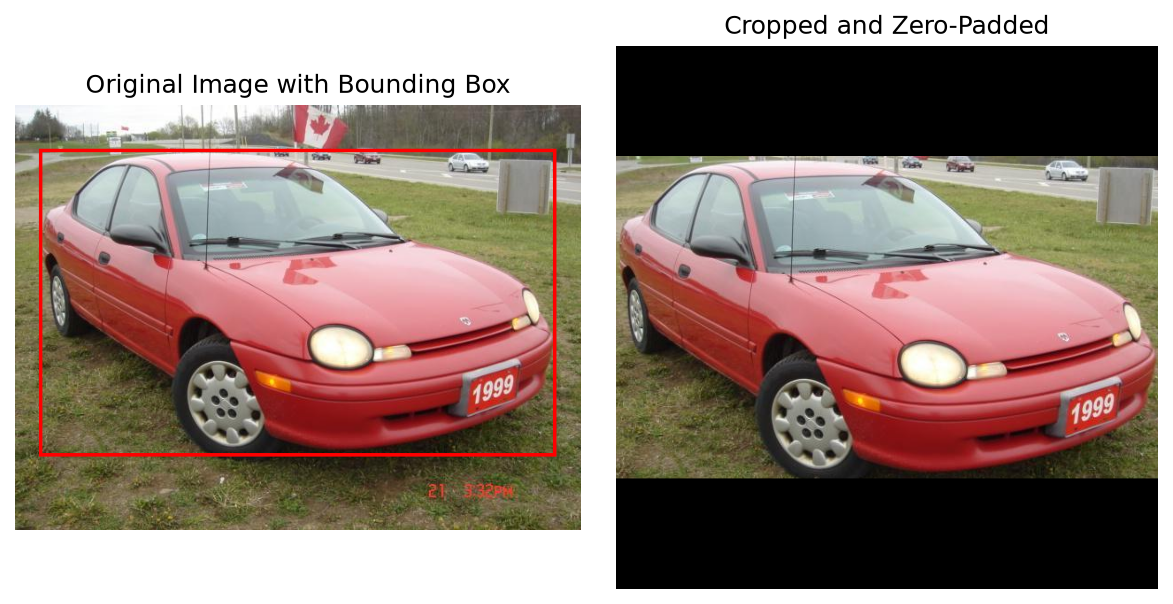
\includegraphics[width=0.45\textwidth]{bbox_preprocessing.png}}
\caption{Data Pre-Processing: The original image with the bounding box in red (left) compared to the final cropped and zero-padded image (right) that is fed into the network.}
\label{fig:bbox}
\end{figure}
\section{Experimental Setup and Transfer Learning}
The image classification pipeline was implemented using the PyTorch deep learning framework. Because training a deep neural network from scratch on a dataset with only 16,185 total images (split between training and testing) would lead to severe overfitting, transfer learning was used. Both the ResNet50 and EfficientNet-B4 models were pre-trained on the massive ImageNet dataset.

\subsection{Two-Phase Training Strategy}
These pre-trained models were adapted for the Stanford Cars dataset using a two-phase training approach:
\begin{enumerate}
    \item \textbf{Phase 1 (Warm-up):} The main body (the backbone) of the network was frozen so its pre-trained weights would not change. Only the final classification layer was trained to learn the 196 specific car classes. This prevents the large initial errors from ruining the good features the network already knew.
    \item \textbf{Phase 2 (Fine-tuning):} After the classification layer stabilized, the entire network was unfrozen. All layers were then trained together using a much smaller learning rate, allowing the model to slowly adjust its feature detection to specifically look for cars instead of general ImageNet objects.
\end{enumerate}

\subsection{Hardware and Reproducibility}
To ensure the results can be replicated, the complete code for data loading, pre-processing, training loops, and evaluation is publicly available on GitHub at [INSERT GITHUB LINK HERE]. 

The training was conducted on a local workstation. Because EfficientNet-B4 uses larger input images (380x380 pixels) compared to ResNet50 (224x224 pixels) and has a more complex structure, it requires significantly more memory. To prevent out-of-memory errors, different batch sizes had to be used. ResNet50 was trained with a batch size of 32, but the batch size had to be reduced to 8 for EfficientNet-B4. The specific hardware used for this experiment was:
\begin{itemize}
    \item \textbf{GPU:} NVIDIA GeForce RTX 3060 Laptop GPU with 6 GB of VRAM.
    \item \textbf{CPU \& RAM:} AMD Ryzen 7 6800H with 16 GB of System RAM.
\end{itemize}
\section{Results and Performance Analysis}
To evaluate the models fairly, they were tested on the official isolated test set of the Stanford Cars dataset. The overall Top-1 accuracy was measured, which means the model only gets credit if its single highest-confidence prediction is exactly correct out of the 196 possible choices.

\subsection{Quantitative Results}
Table \ref{tab:results} summarizes the final test accuracy for both models. EfficientNet-B4 significantly outperformed ResNet50. This improvement is expected because EfficientNet uses a more advanced architecture and processes images at a much higher resolution (380x380 compared to 224x224), which is crucial for finding the tiny details needed in fine-grained classification.

It is important to note that both models were trained for exactly 40 epochs. While ResNet50's validation accuracy plateaued around the 30th epoch (hovering near 80\% for the final 10 epochs), EfficientNet-B4 was still showing signs of improvement. However, training for EfficientNet-B4 was halted at 40 epochs due to hardware and time constraints. This suggests that the performance gap between the two models could potentially be even wider if EfficientNet-B4 were allowed to train until complete convergence.

\begin{table}[htbp]
\caption{Final Test Set Accuracy}
\begin{center}
\begin{tabular}{|c|c|c|c|}
\hline
\textbf{Model} & \textbf{Input Size} & \textbf{Top-1 Accuracy} \\
\hline
ResNet50 & 224x224 & 80.59\% \\
\hline
EfficientNet-B4 & 380x380 & 82.39\% \\
\hline
\end{tabular}
\label{tab:results}
\end{center}
\end{table}

\subsection{Error Analysis}
To understand where the models make mistakes, confusion matrices were generated for both ResNet50 and EfficientNet-B4 (Figures \ref{fig:conf_resnet} and \ref{fig:conf_effnet}). Displaying a full 196x196 matrix can be visually overwhelming, so both the complete macroscopic view and a focused subset of the first 20 classes are provided for each model.

The dark diagonal line across the full matrices indicates that both models correctly classify the majority of the dataset. By examining the 20-class subsets, it becomes clear that when the models do make mistakes, the confusion usually happens between cars of the same make or similar visual characteristics (e.g., there is notable confusion between Class 15, the Audi R8 Coupe 2012, and Class 16, the Audi V8 Sedan 1994). When comparing the two, EfficientNet-B4 displays slightly less off-diagonal spread, confirming its higher accuracy.

\begin{figure}[htbp]
\centerline{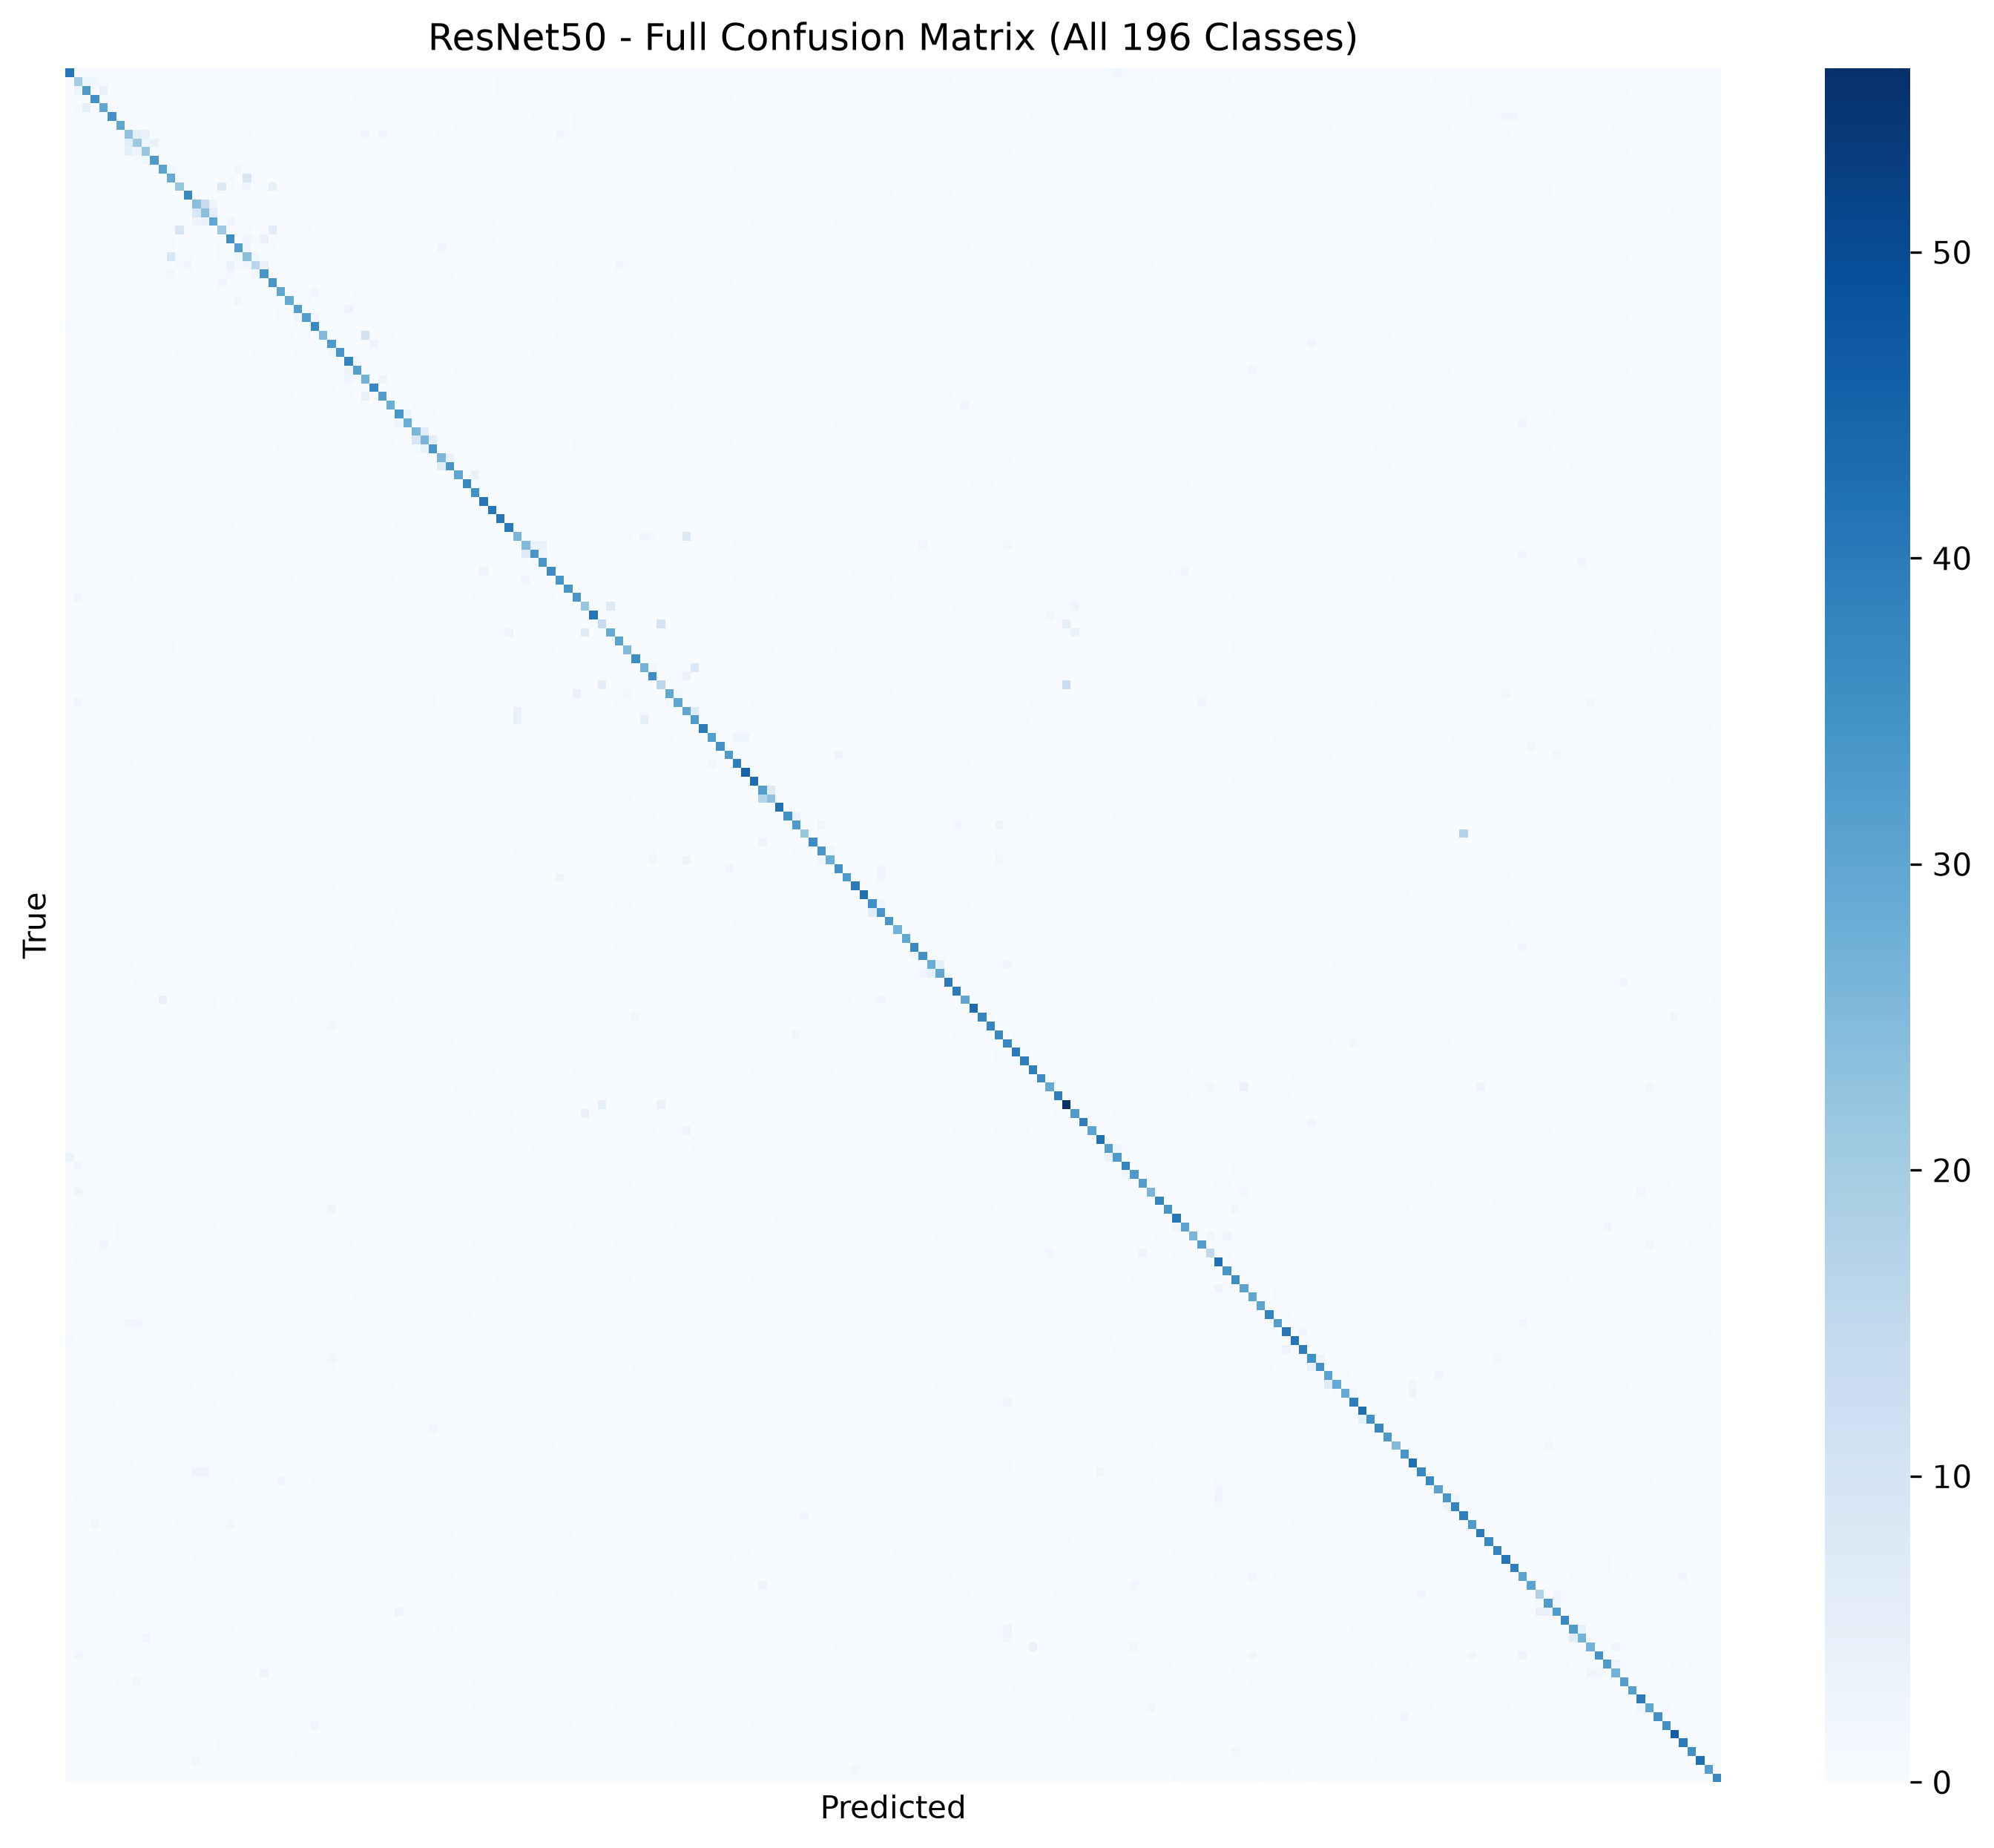
\includegraphics[width=0.45\textwidth]{resnet_matrix_full.png}}
\vspace{0.2cm}
\centerline{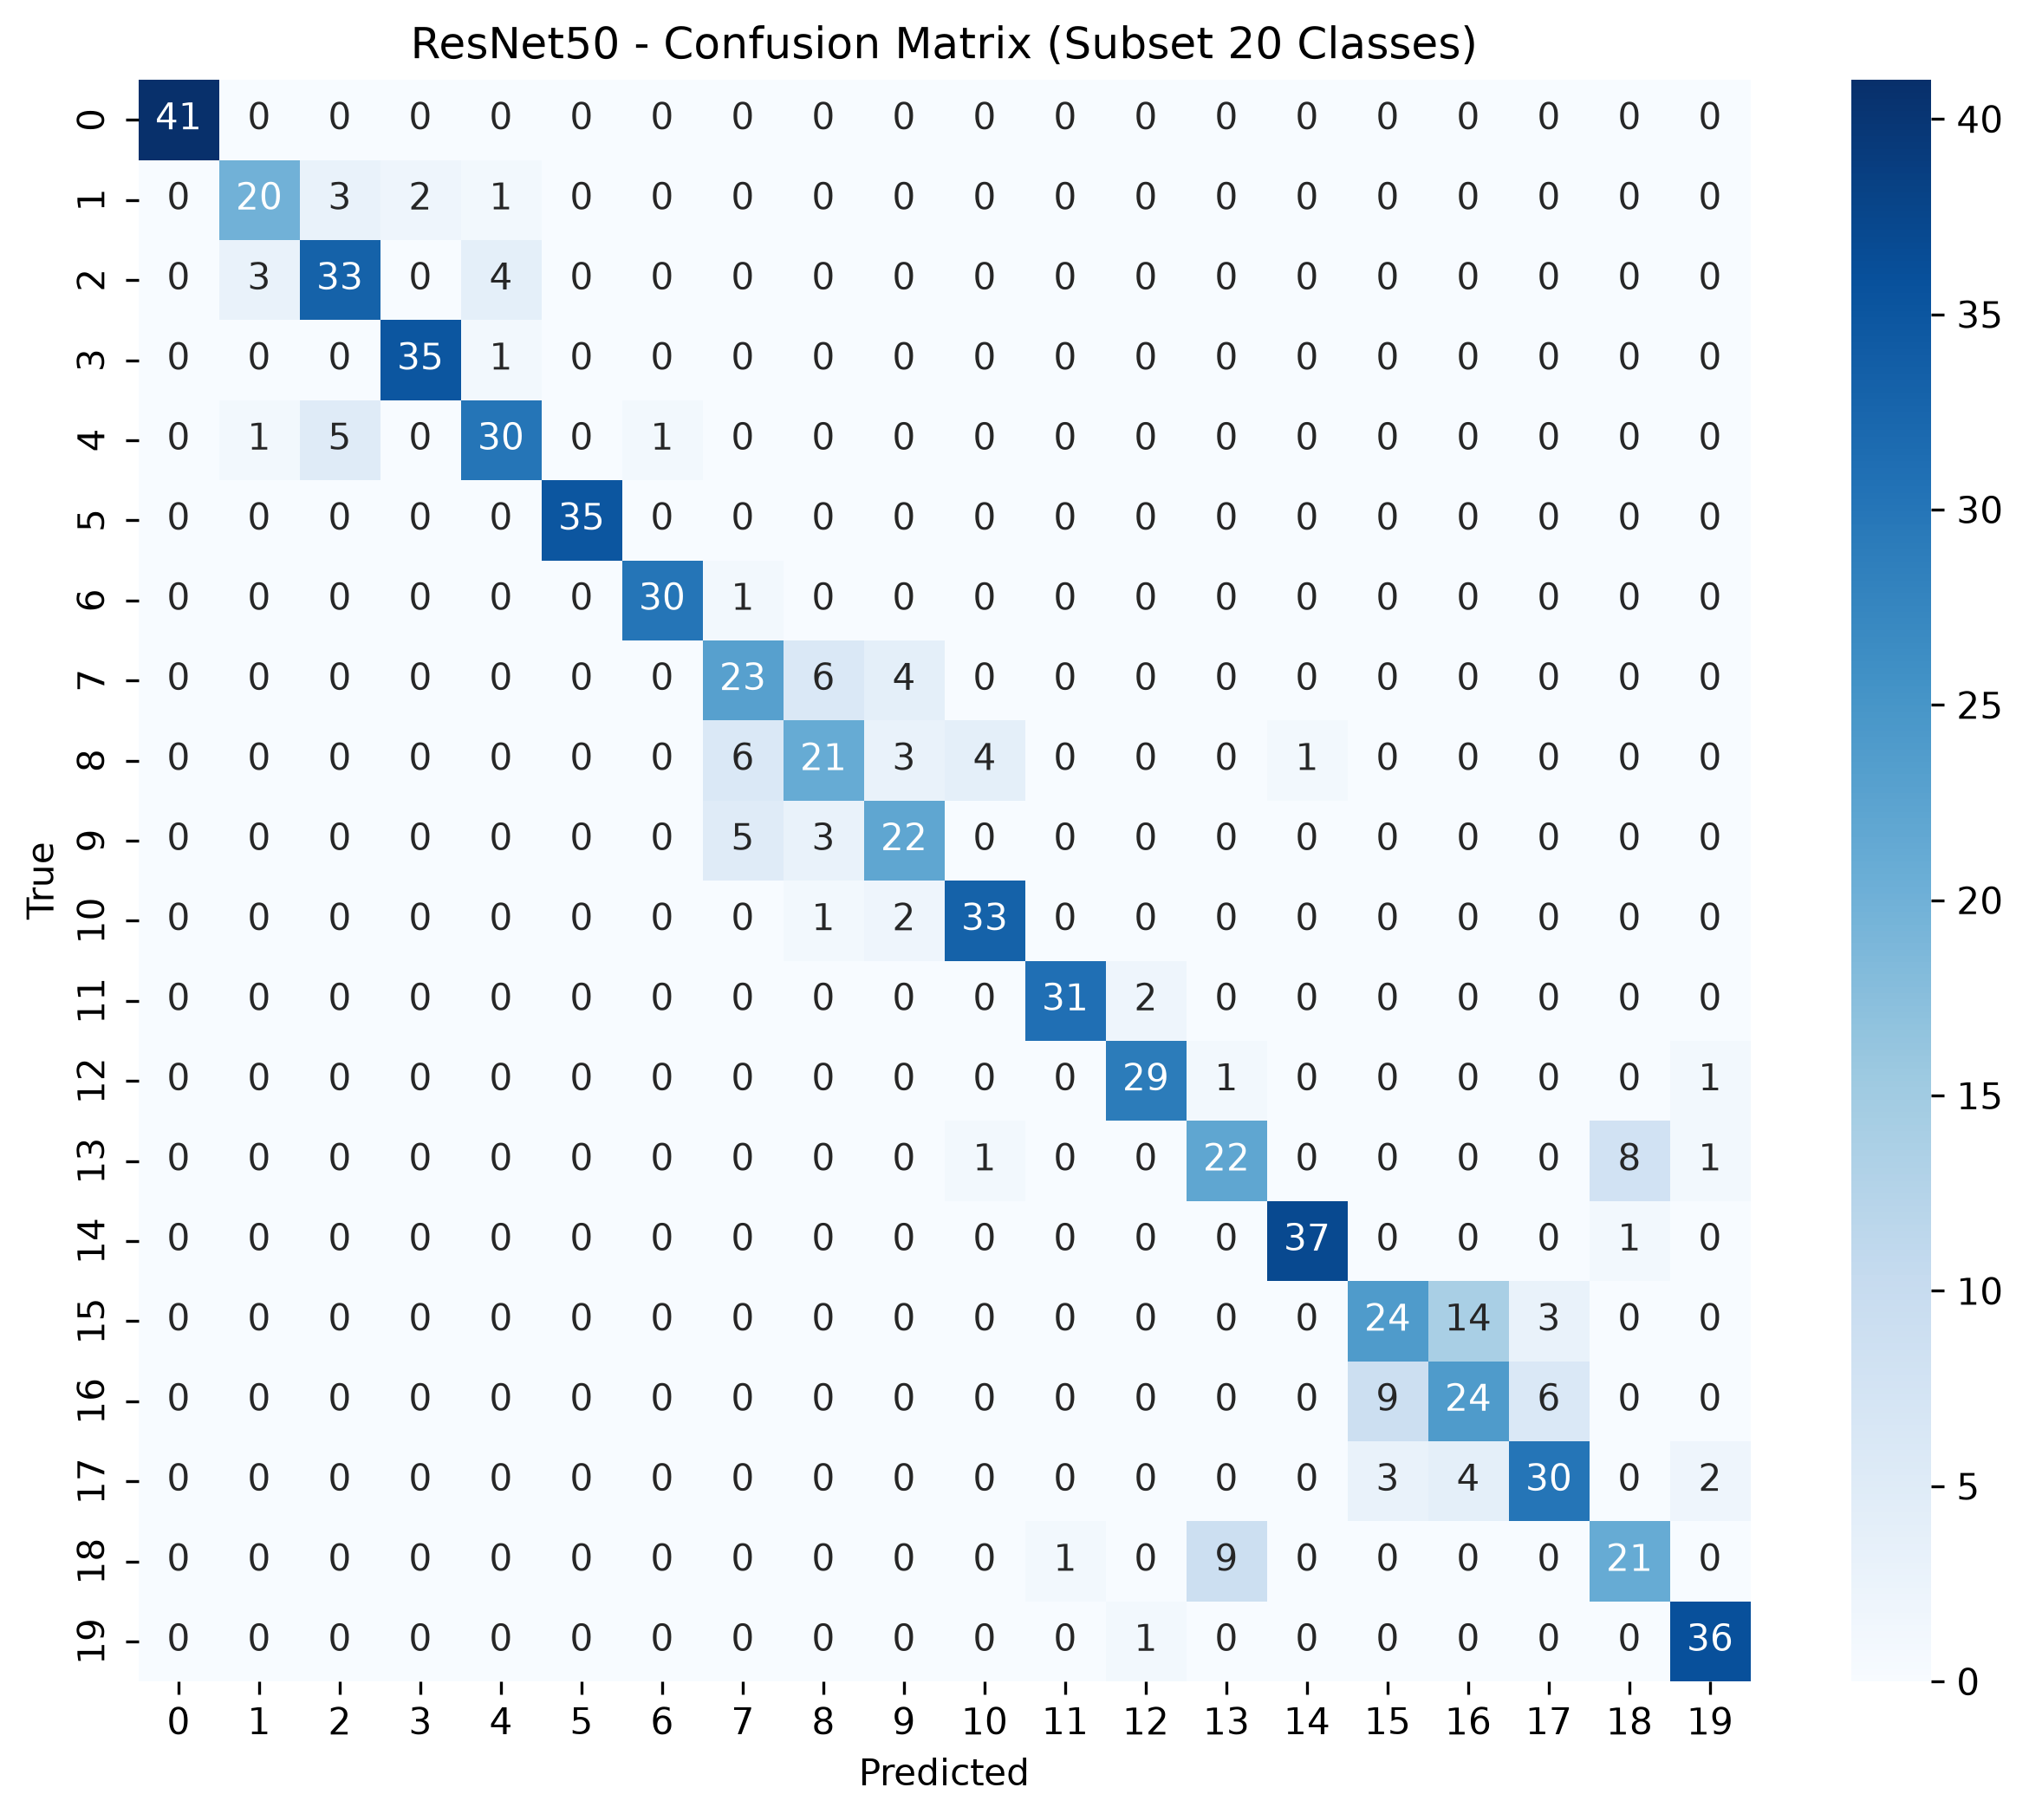
\includegraphics[width=0.45\textwidth]{resnet_matrix_subset.png}}
\caption{ResNet50 Confusion Matrices. Top: Full 196-class matrix showing overall diagonal dominance. Bottom: Focused 20-class subset highlighting inter-class confusion between similar years.}
\label{fig:conf_resnet}
\end{figure}

\begin{figure}[htbp]
\centerline{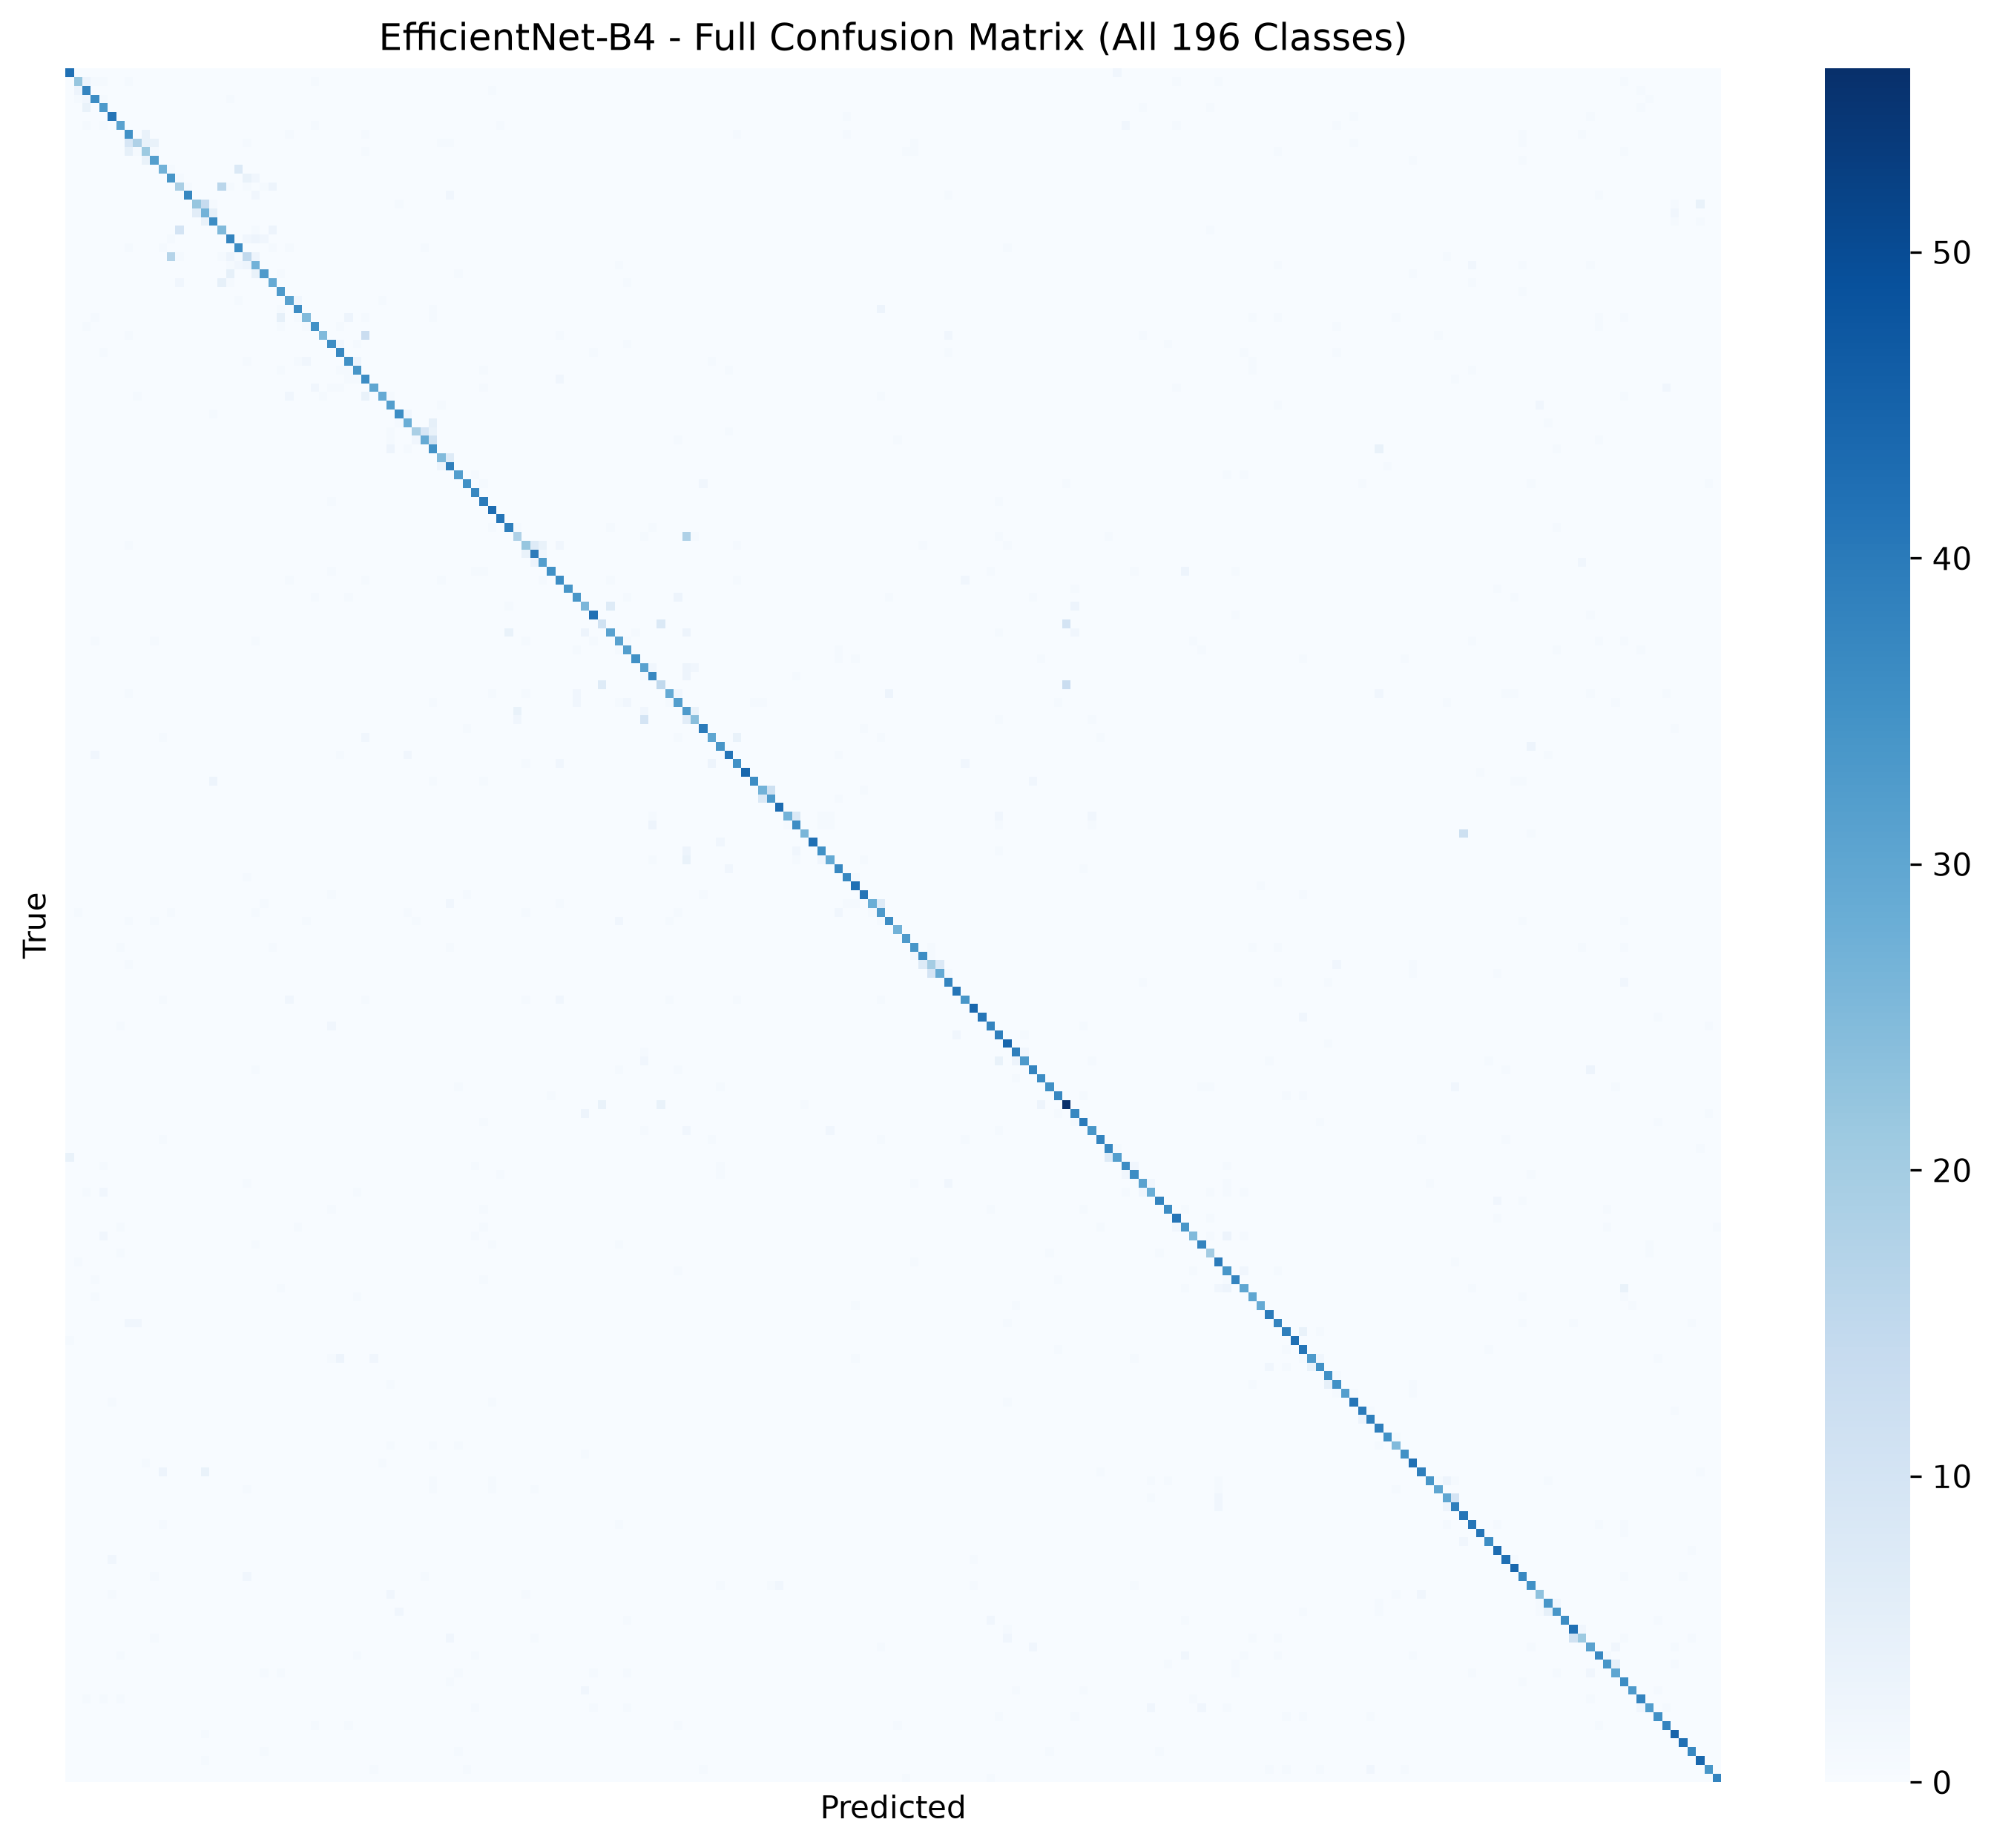
\includegraphics[width=0.45\textwidth]{effnet_matrix_full.png}}
\vspace{0.2cm}
\centerline{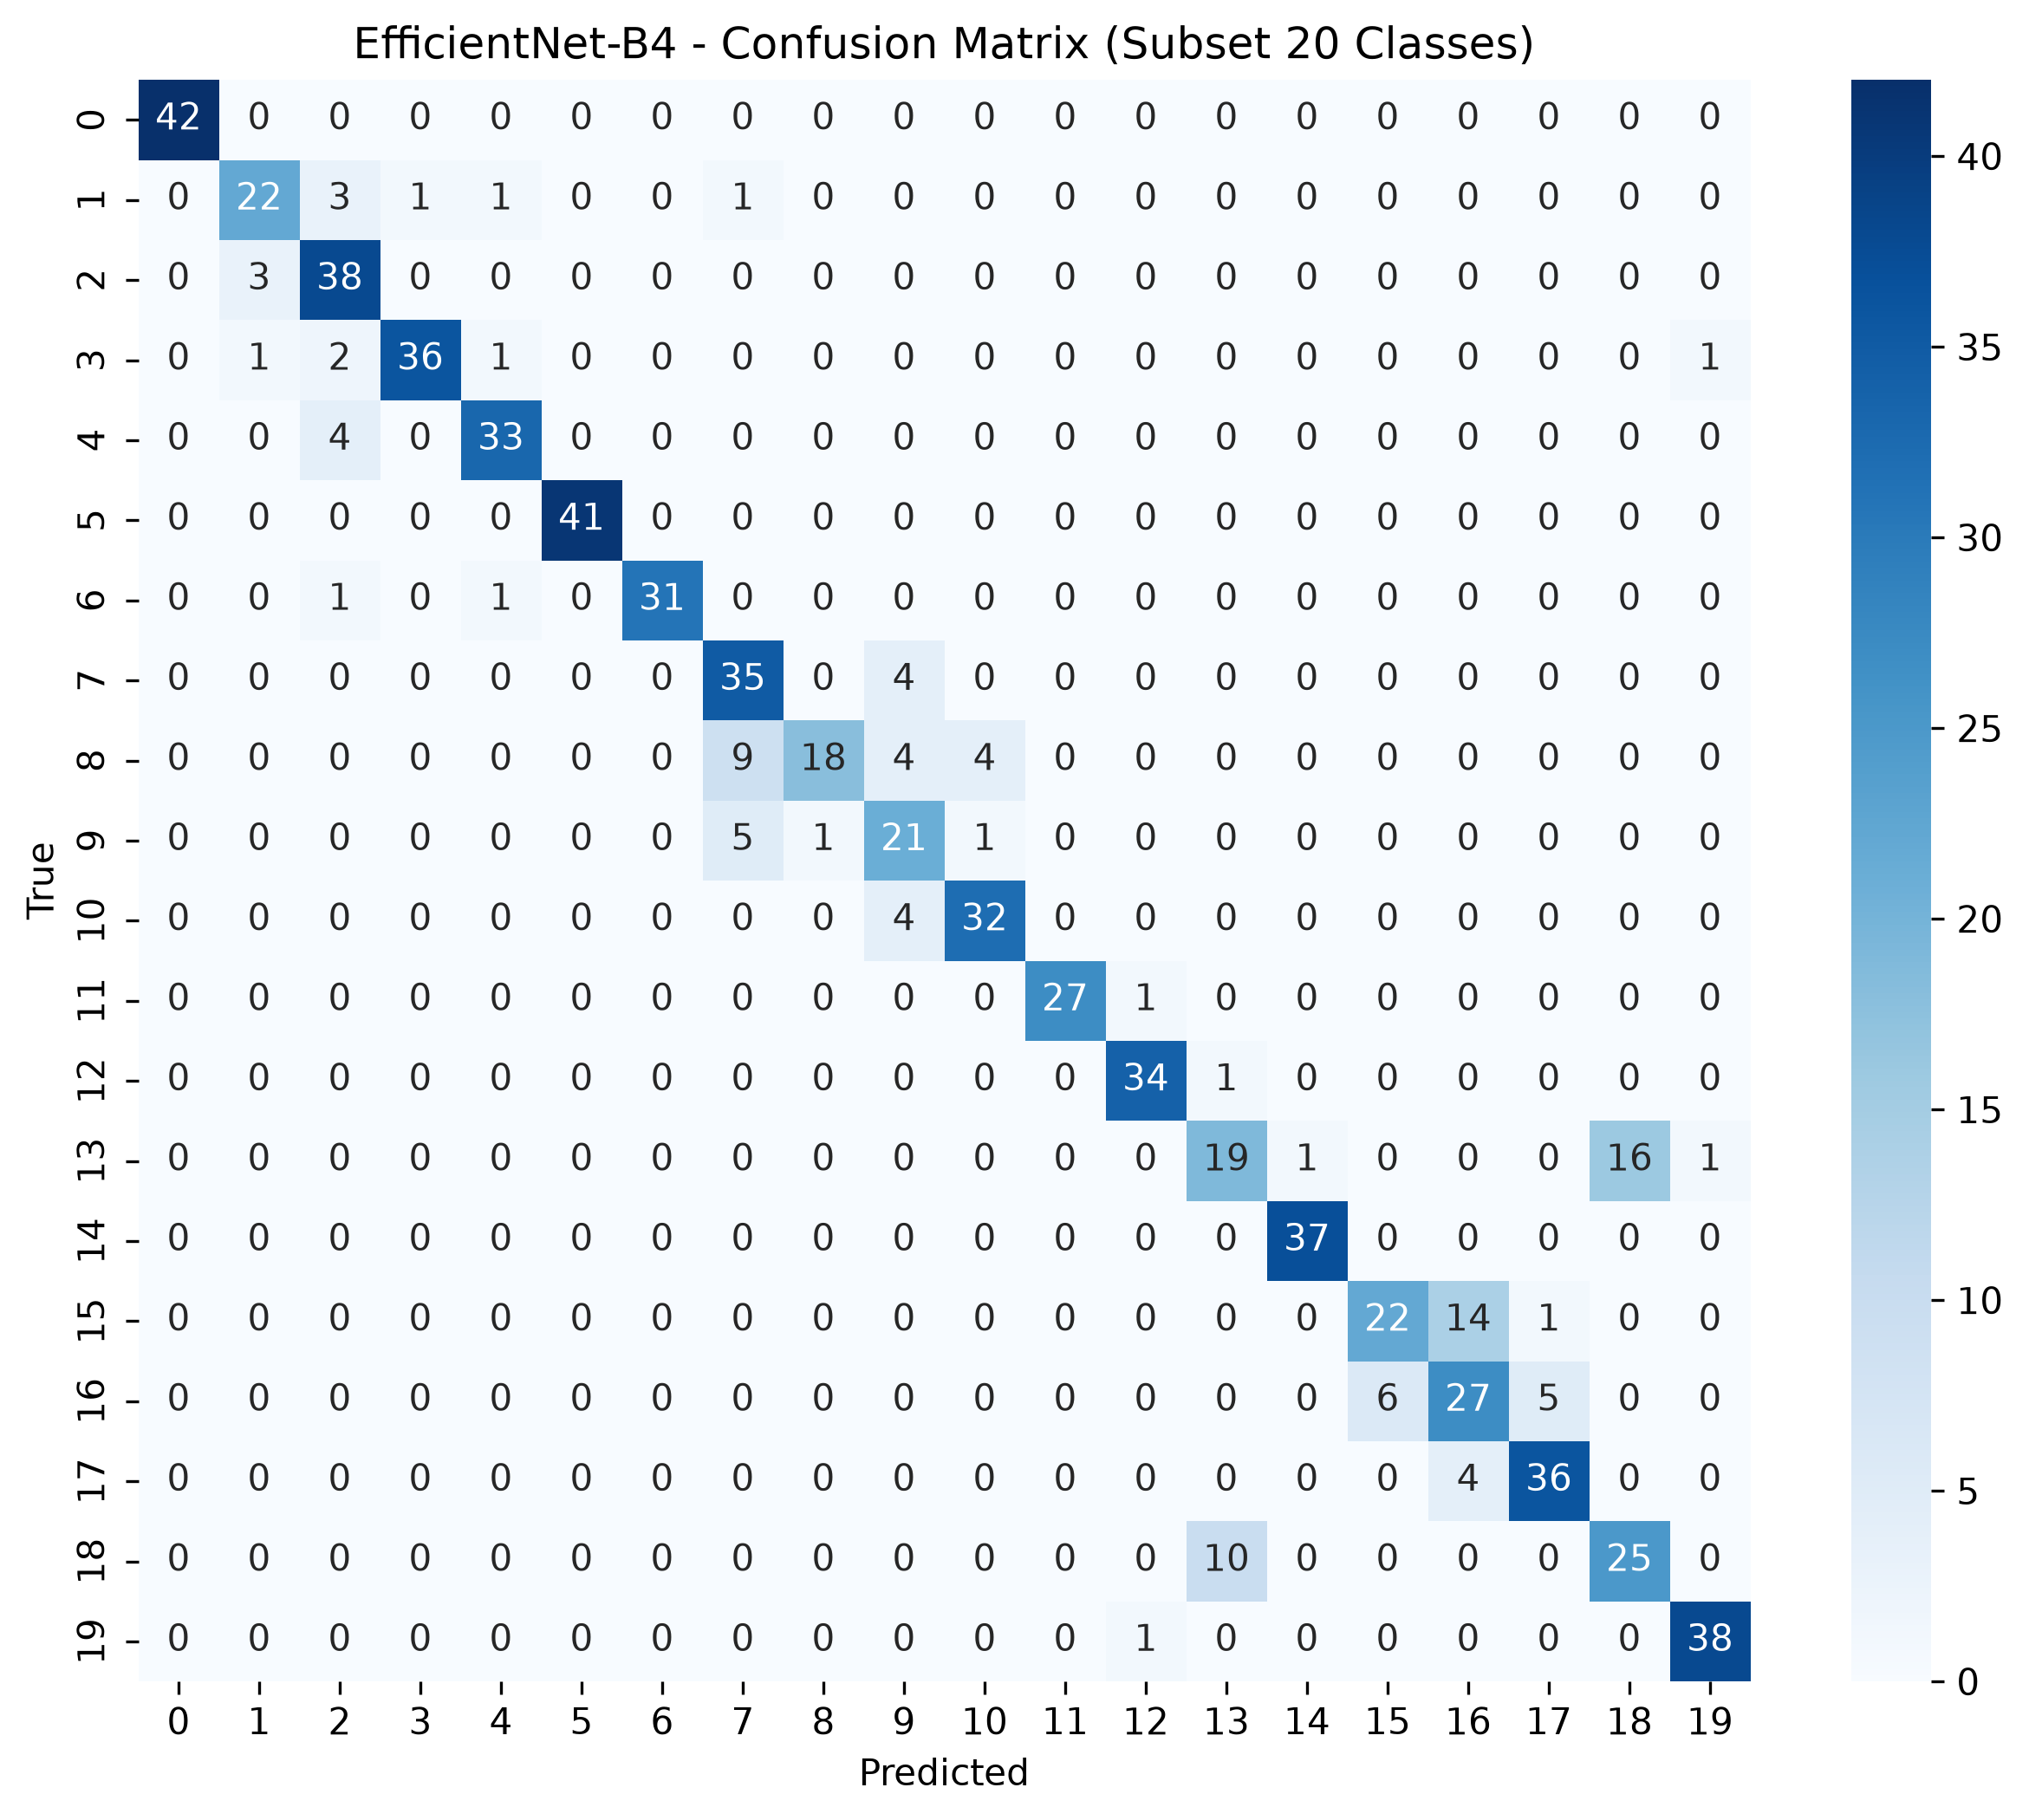
\includegraphics[width=0.45\textwidth]{effnet_matrix_subset.png}}
\caption{EfficientNet-B4 Confusion Matrices. Top: Full matrix. Bottom: Focused 20-class subset, demonstrating sharper predictions compared to ResNet50.}
\label{fig:conf_effnet}
\end{figure}
\section{Interpretability and The Padding Artifact}
To ensure the models were actually looking at the cars and not cheating by finding hidden clues in the background, a technique called Grad-CAM (Gradient-weighted Class Activation Mapping) was used. Grad-CAM creates a heatmap over the original image, highlighting the exact regions the neural network focused on to make its decision. Red regions indicate high importance, while blue regions indicate low importance.

\subsection{Discovering the Padding Artifact}
When analyzing the Grad-CAM heatmaps for both ResNet50 and EfficientNet-B4, an unexpected behavioral pattern was observed. As expected, the networks focused heavily on distinguishing features like headlights, grilles, and the shape of the windows. However, they also consistently highlighted the black zero-padding borders added during the letterboxing pre-processing step.

At first, this seemed like a flaw. Why would the network look at empty black pixels? Upon further analysis, it was realized the networks had learned to use the padding thickness as a clever geometric shortcut. Because a long vehicle (like a pickup truck) requires very thick horizontal padding to become a square, and a tall vehicle (like an SUV) requires vertical padding, the black bars act as a direct indicator of the car's original aspect ratio. This behavior aligns with recent findings by Islam et al. \cite{islam2020position}, who demonstrated that CNNs exploit zero-padding to implicitly encode absolute spatial and geometric information.

To illustrate this, two scenarios are presented. Figure \ref{fig:gradcam_good} shows examples where both models predict correctly by focusing heavily on expected car features (e.g., the grille and headlights of an Audi). In contrast, Figure \ref{fig:gradcam_bad} shows failure cases where both models predict incorrectly. In these bad examples, it is highly noticeable that EfficientNet-B4 shifts its attention away from the car itself and shows intense activation maps along the black zero-padding borders, attempting to use the artificial bounding box rather than the visual features to guess the class.

\begin{figure}[htbp]
\centerline{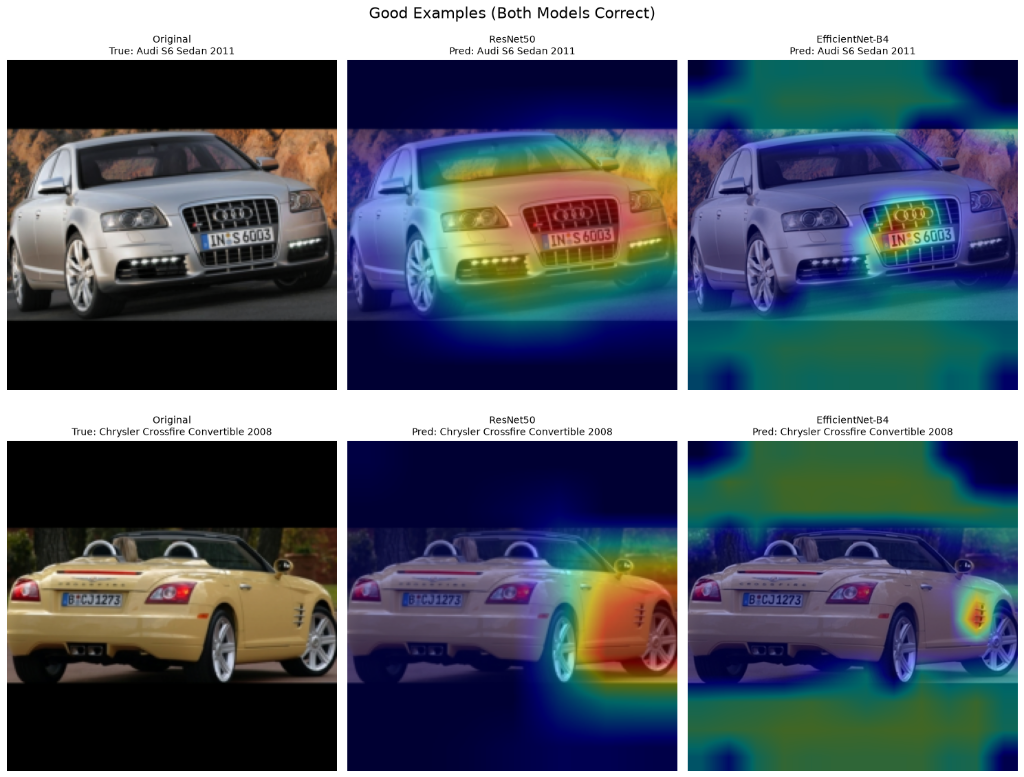
\includegraphics[width=0.48\textwidth]{gradcam_good.png}}
\caption{Grad-CAM visualization of successful predictions. Both ResNet50 (middle) and EfficientNet-B4 (right) focus heavily on discriminative car features such as headlights, grilles, and distinct body shapes.}
\label{fig:gradcam_good}
\end{figure}

\begin{figure}[htbp]
\centerline{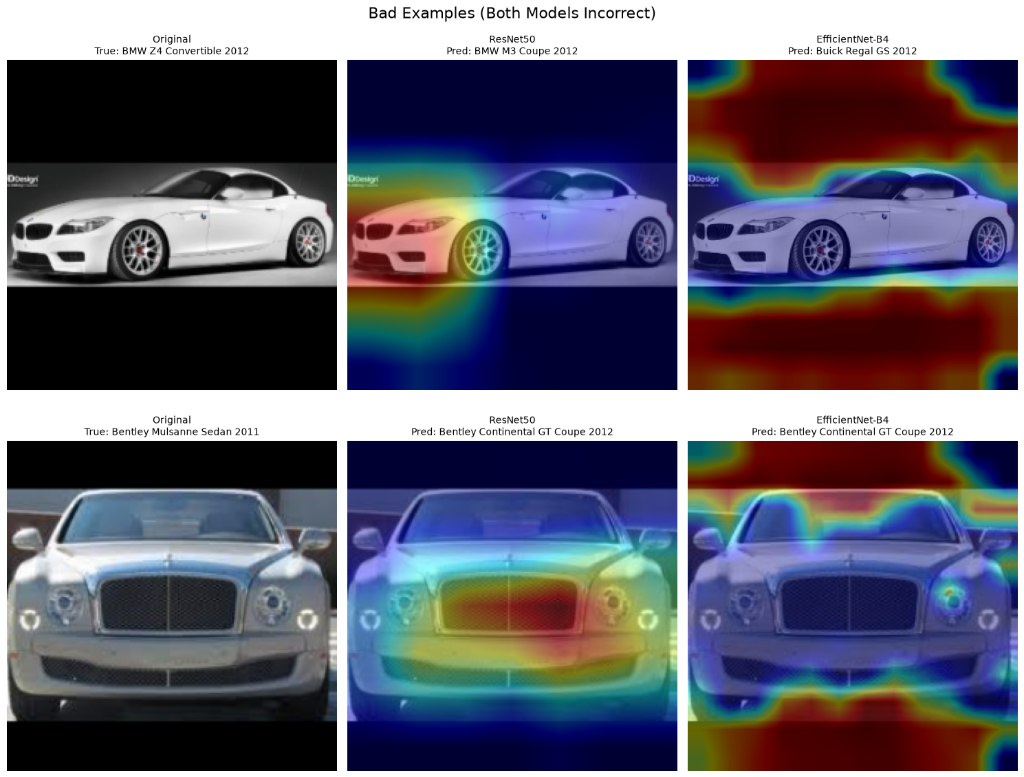
\includegraphics[width=0.48\textwidth]{gradcam_bad.png}}
\caption{Grad-CAM visualization of incorrect predictions demonstrating the padding artifact. Notice how EfficientNet-B4 (right column), in particular, shows intense activation along the black zero-padding borders, attempting to use the artificial geometric boundaries rather than the car's actual textures to make a prediction.}
\label{fig:gradcam_bad}
\end{figure}

This is a classic example of neural networks finding the path of least resistance. Instead of only learning complex textures, the models learned that measuring the black padding is an easy and highly accurate way to eliminate categories of cars with different physical dimensions.
\section{Conclusion}
In this project, the challenge of fine-grained vehicle classification using the Stanford Cars dataset was explored. A standard ResNet50 model was compared against a more modern EfficientNet-B4 architecture. By utilizing a two-phase transfer learning strategy, strong results were achieved despite the dataset's small size. EfficientNet-B4 achieved a higher accuracy of 82.39\% compared to ResNet50's 80.59\%, proving that higher resolution inputs and optimized scaling lead to better fine-grained feature detection. This performance was achieved under a strict 40-epoch training limit, suggesting EfficientNet-B4 could reach even higher accuracy if not restricted by hardware constraints.

Furthermore, the use of Grad-CAM visualization revealed an unintended but fascinating behavior: the models learned to use the zero-padding pre-processing step to determine the vehicle's aspect ratio. This highlights the importance of not only looking at accuracy metrics, but also investigating how and why deep learning models make their decisions. Future work could involve cropping the images differently or using more advanced data augmentation to prevent the model from relying on these artificial borders.

\begin{thebibliography}{00}
\bibitem{krause20133d} J. Krause, M. Stark, J. Deng, and L. Fei-Fei, `3D object representations for fine-grained categorization,'' in \textit{Proceedings of the IEEE International Conference on Computer Vision Workshops}, 2013, pp. 554--561.
\bibitem{he2016resnet} K. He, X. Zhang, S. Ren, and J. Sun, `Deep residual learning for image recognition,'' in \textit{Proceedings of the IEEE Conference on Computer Vision and Pattern Recognition}, 2016, pp. 770--778.
\bibitem{tan2019efficientnet} M. Tan and Q. Le, `EfficientNet: Rethinking model scaling for convolutional neural networks,'' in \textit{International Conference on Machine Learning}, 2019, pp. 6105--6114.
\bibitem{cleanlab_cars} Cleanlab, `Stanford Cars Dataset Analysis,'' 2024. [Online]. Available: https://cleanlab.ai
\bibitem{sota_vit} Papers with Code, `Stanford Cars Benchmark,'' 2024. [Online]. Available: https://paperswithcode.com/dataset/stanford-cars
\bibitem{islam2020position} M. A. Islam, S. Jia, and N. D. B. Bruce, `How much position information do convolutional neural networks encode?'' in \textit{International Conference on Learning Representations}, 2020.
\end{thebibliography}

\end{document}